% !TeX spellcheck = en_GB
% encoding: utf8
% !TEX encoding = utf8
% !TEX program = pdflatex
% !BIB program = biber

\documentclass[11pt,oneside,a4paper]{report}

\usepackage[utf8]{inputenc}
\usepackage[T1]{fontenc}
\usepackage[colorlinks]{hyperref}
\usepackage[left=2.5cm, right=2.5cm, top=2.5cm, bottom=2.5cm]{geometry}
\usepackage{float}
\usepackage{subcaption}
\usepackage{mathtools}
\usepackage{color}
\usepackage{listings}
\usepackage{xcolor}
\usepackage[backend=biber,maxnames=10,style=numeric,sorting=nty,abbreviate=false,giveninits=true,language=english]{biblatex}

\addbibresource{../meros.bib}

%\newcommand{\twc}[1]{\textcolor{red}{\textbf{TW}: #1}}
\newcommand{\Fig}[1]{Fig.~\ref{#1}}

\definecolor{amber}{rgb}{1.0, 0.49, 0.0}
\newcommand{\twci}[1]{
	\textcolor{amber}{TW: #1}}

% encoding: utf8
%
% Stereotypes
%

% Lista powinna być zgodna z profilem w EA

\newcommand{\stActionConn}{<<Action>>}
\newcommand{\stCommChannel}{<<CommChannel>>}
\newcommand{\stComponContain}{<<ComponContain>>}
\newcommand{\stGpPackages}{<<GpPackages>>}
\newcommand{\stHardware}{<<Hardware>>}
\newcommand{\stLaunchFile}{<<LaunchFile>>}
\newcommand{\stMetaPackage}{<<MetaPackage>>}
\newcommand{\stMicroNode}{<<MicroNode>>}
\newcommand{\stNamespace}{<<Namespace>>}
\newcommand{\stNode}{<<Node>>}
\newcommand{\stPackage}{<<Package>>}
\newcommand{\stParameter}{<<Parameter>>}
\newcommand{\stRepository}{<<Repository>>}
\newcommand{\stRosCommCompon}{<<RosCommCompon>>}
\newcommand{\stRosConn}{<<RosConn>>}
\newcommand{\stRQtNode}{<<RQtNode>>}
\newcommand{\stRunSystemCompon}{<<RunSystemCompon>>}
\newcommand{\stServiceConn}{<<Service>>}
\newcommand{\stSourExeContain}{<<SourExeContain>>}
\newcommand{\stSystem}{<<System>>}
\newcommand{\stTerminal}{<<Terminal>>}
\newcommand{\stTopicConn}{<<Topic>>}
\newcommand{\stWorkspace}{<<Workspace>>}

\newcommand{\stblock}{<<block>>}






\lstdefinestyle{terminal}{
	backgroundcolor=\color{darkgray},
	basicstyle=\ttfamily\color{green}\footnotesize,
	frame=single,
	rulecolor=\color{gray},
}


\begin{document}
	
\title{MeROS: basics of metamodel usage with turtlesim}
\author{MeROS developers group - https://github.com/twiniars/MeROS \\ tomasz.winiarski@pw.edu.pl}
\date{\today}
\maketitle

	
	
	\maketitle
	

	
\chapter*{Important citation notice}

\textbf{If you are to use MeROS in your papers, please first cite the IEEE ACCESS  article~\cite{meros-access}, where the initial version of the MeROS is presented. You can also refer to MeROS project page \cite{meros-www} and mention the actual MeROS version you are using.}
	
\chapter{Introduction}
\label{ch:introduction}

	This document is to present basics of MeROS metamodel usage (its application). It bases on popular turtlesim ROS2 tutorial \url{https://docs.ros.org/en/jazzy/Tutorials/Beginner-CLI-Tools.html} and has an introspection, reverse engineering nature. The procedure of the new systems creation with V-model and MerROS is presented in \cite{winiarski2025-v-model}. We advice to read it after this documentation as the article adds a lot of valuable examples of MeROS related diagrams creation. 

\chapter{MeROS application}
\label{ch:application}
Scenariusz - raczej do usuniecia na koniec:
\begin{itemize}
	\item Zaczynamy od określenia ogólnego działania systemu. Pierwszy sd ma charakter ogolny z operatorem i Systemem. Operator wysyla polecenia ruchu do przodu i robot jedzie do przodu. Potem wysyla na akcji polecenie oborotu do pozycji aboslutnej i system to wykonuje.
	\item powołujemy system z turtlesim i teleop turtle
	\item rysujemy rqt\_graph z wylaczonymi wszystkimi extra opcjami. Zaczłączamy ten rysunek w tej dokumentacji
	\item Zaznaczamy, że system prezentuje te elementy i zachowania, ktore sa istotne z punktu widzenia prezentowanego przykladu
	\item Pakiety dla nodow z rqt\_graph  znamy, bo do ich uruchomienia potrzebowalismy je podac. Co wiecej mozemy to sprawdzic poleceniem ros2 pkg executables turtlesim
	\item sprawdzamy ros2 node info interesujace nas pakiety dla metod komunikacji
	\item rysujemy diagram dla workspace z pakietami z nodami i pakietami z metodami komunikacji. Nawy nodow i metod komunikacji z nazwa pakietu. Uzywamy podwojengo dwukropka w srodku w nazwach nodow z pakietami i analogicznie dla metod komunikacji.
	\item Potem rysujmy diagram bdd dla uruchomionego systemu. Musi on bezposrednio agrogowac nody i kanal komunikacyjny. W skład kanału komunikacyjngo metody komunikacyjne. Pytanko jak zapewnic uniwersalnosc kanalu komunikacyjnego - jakies uniwersalne etykiety komponentow komunikujacych się na bokac?
	\item Rysujemy diagram ibd dla bdd powyzej. Może Kanał zdefiniowany powyżej, a nie dalej?
	\item Bdd i ibd dla kanału komunikacyjnego.
	\item Podsumowujący diagram sekwencji ma charakter szczegolowy. Tu sa juz wciskane konkretne przyciski i pojawiaja sie zamiast Systemu jego komponenty takie jak nody, topiki i akcje. Można pokazać trzy zrzuty okna z zolwiem w roznych fazach wykonania zadania. Jakoś to trzeba zmapowac na chwile czasowe z diagramu sd.
\end{itemize}















The MeROS \stSystem{} structure presentation is composed by different views on it. In this example we start with Sources and Executables composition into the System. It should be noted that tourtlesim package should be installed before as well as  source command should be executed properly in each system console.

\begin{lstlisting}[style=terminal]
$ ros2 pkg executables turtlesim
turtlesim draw_square
turtlesim mimic
turtlesim turtle_teleop_key
turtlesim turtlesim_node
\end{lstlisting}

There are four executables in the turtlesim \stPackage{} that can be treated as \stNode{}s. They are composed into the ROS 2 \stWorkspace{} localised in /opt directory (Fig.~\ref{fig:system_sourexec_composition_bdd}).


\begin{figure}[H]
	\centering
	\begin{center}
		{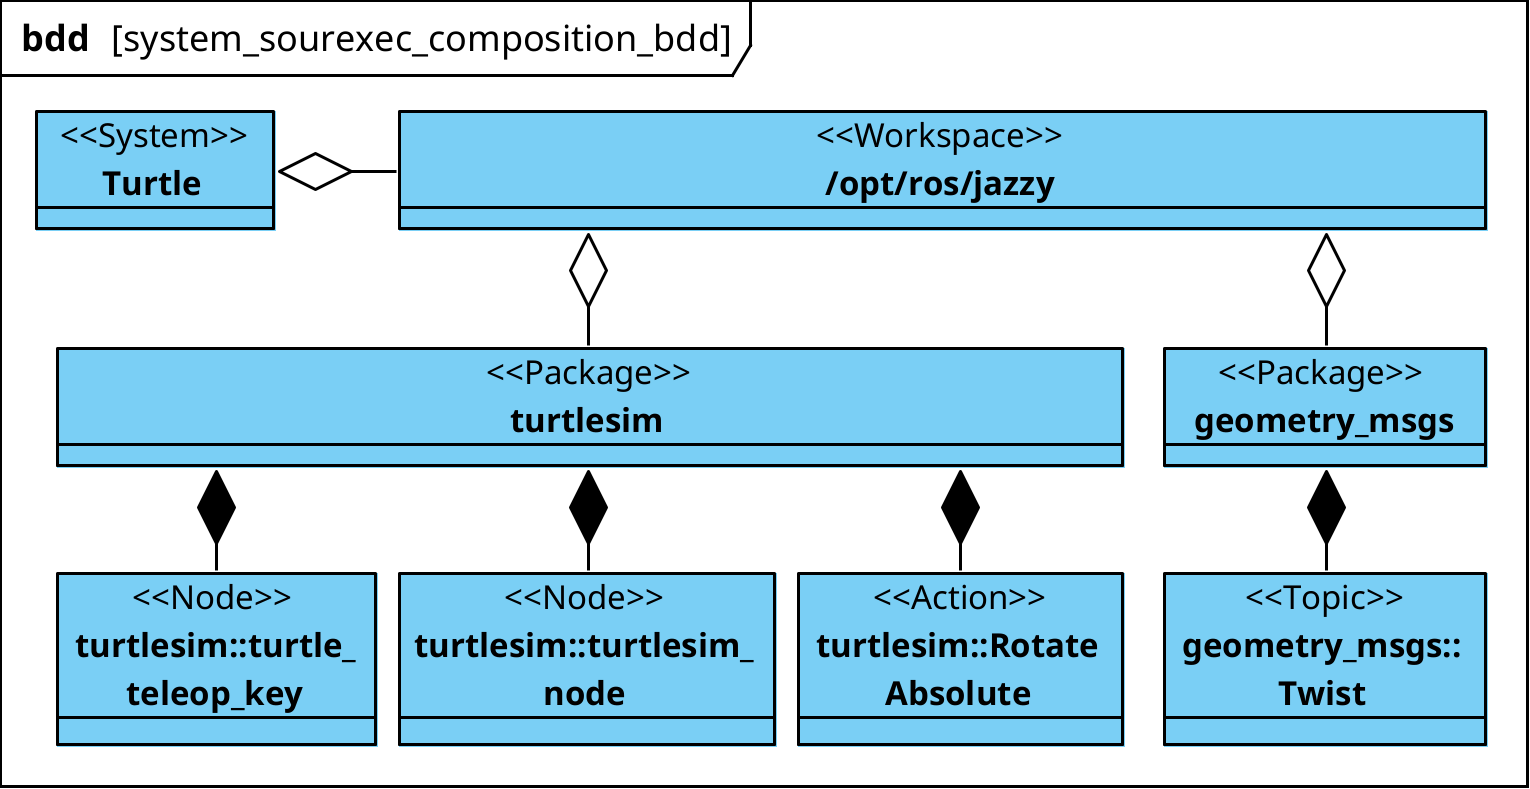
\includegraphics[scale=1.0]{diagrams/system_sourexec_composition_bdd.png}}
	\end{center}
	\caption{System sources and executables composition}
	\label{fig:system_sourexec_composition_bdd}
\end{figure}


			
\AtNextBibliography{\small}
\printbibliography
	
\end{document}
